\providecommand{\main}{../../main}
\documentclass[../../main/main.tex]{subfiles}


\begin{document}

\section{Experimental data analysis and results}
After having performed all the tests for the setup characterisation, we discuss in this Section the technical details of the final measurements for the scattering process and then we treat the analysis of the acquired data. Lastly, we present the methods employed to extract meaningful results from the measurements and, to conclude, we discuss their significance.



\subsection{Data acquisition planning}
Using the information provided by the numerical simulation of the scattering process, we have planned a series of acquisitions of different duration, depending on the angular position of the detector with respect to the beam centre.
Aside from the time extension of the acquisitions, there are other parameters to take into account for a correct execution of this part of experiment. In particular, for every angle:
\begin{itemize}
    \item we should set a reasonable number of memory blocks for the SSB acquisition system, in order to make the dead time correction negligible;
    \item we must choose an optimal configuration of strobe and gap values for the ALPIDE detector, in order to avoid the overflow of the FIFO pipeline and the consequent corruption of the acquired data.
\end{itemize}
More precisely, for the SSB detector we identify five regions and for each of these we establish an angular interval of acquisition and the number memory blocks to use.
On the other hand, for ALPIDE detector, due to its wider angular opening, we acquire at regular intervals, selecting each time the correct combination of the aforementioned parameters.
A brief summary of the position, duration and parameters of the acquisitions is reported in \tabref{tab:tempiPICO} and \tabref{tab:tempiALPIDE} for both SSB and ALPIDE detection systems.


\begin{table}[h]
    \begin{tabular}{cccc}
        \toprule
        \multicolumn{4}{c}{\small \bf SSB detector}  \\
        \colrule
        \textbf{Angle [deg]}    &
        \textbf{Sampling interval [deg]}   &
        \textbf{Samples per block}  &
        \textbf{\boldmath Programmed \( t_{\mathrm{acq}} \) [h]}    \\
        \colrule
        \( \abs{\theta} \in [ 0.0,  9.0[ \)   &   \(  2 \)  &   \( 100 \)    &    \(   1 \)   \\
        \( \abs{\theta} \in [ 9.0, 18.0[ \)   &   \(  2 \)  &   \(  10 \)    &    \(   4 \)   \\
        \( \abs{\theta} \in [18.0, 27.0[ \)   &   \(  2 \)  &   \(   1 \)    &    \(   8 \)   \\
        \( \abs{\theta} \in [27.0, 36.0[ \)   &   \(  5 \)  &   \(   1 \)    &    \(  24 \)   \\
        \( \abs{\theta} \in [36.0, 54.0[ \)   &   \( 10 \)  &   \(   1 \)    &    \(  72 \)   \\
        \botrule
    \end{tabular}
    \caption{Programmed acquisition times for each angular region for SSB detection system, along with the corresponding chosen number of memory blocks for dead time reduction.}
    \label{tab:tempiPICO}
\end{table}

% \begin{table}[h]
%     \begin{tabular}{l|ccccc}
%         \toprule
%         \multicolumn{6}{c}{\small \bf SSB Detector}  \\
%         \colrule
%         \textbf{Region [deg]}  & $|\theta|\in [0,9.0[ $ & $|\theta|\in [9.0,18.0[$ & $|\theta|\in [18.0,27.0[$ & $|\theta|\in [27.0,36.0[$
%         & $|\theta|\in [36.0,54.0]$ \\
%         \textbf{Interval [deg]}  & 2  & 2 & 2 &5 & 10 \\
                            
%         \textbf{Samples per Block}  & 100 & 10 & 1  &1 & 
%                                         1 \\            
       
%         \textbf{\boldmath Programmed \( t_{\mathrm{acq}} \) [h]} & 1 & 4 & 8  & 24 & 
%                                       72 \\
%         \botrule
        
%     \end{tabular}
%     \caption{Acquisition time and parameters selected.}
%     \label{tab:tempiPICO}
% \end{table}



\begin{table}[h]
    \begin{tabular}{cccc}
        \toprule
        \multicolumn{4}{c}{\small \bf ALPIDE detector}  \\
        \colrule
        \textbf{Angle [deg]}    &
        \textbf{\boldmath Strobe [$10^3$ clk cycles]}   &
        \textbf{\boldmath Gap [$10^3$ clk cycles]}  &
        \textbf{\boldmath Programmed \( t_{\mathrm{acq}} \) [h]}    \\
        \colrule
        \( \pm  0   \)   &   \(  5 \)  &   \( 65 \)    &    \(  1 \)   \\
        \( \pm  9.0 \)   &   \(  5 \)  &   \( 65 \)    &    \(  2 \)   \\
        \( \pm 18.0 \)   &   \(  5 \)  &   \( 45 \)    &    \(  4 \)   \\
        \( \pm 27.0 \)   &   \(  5 \)  &   \( 25 \)    &    \( 12 \)   \\
        \( \pm 36.0 \)   &   \(  5 \)  &   \( 25 \)    &    \( 24 \)   \\
        \( \pm 45.0 \)   &   \(  5 \)  &   \( 25 \)    &    \( 48 \)   \\
        \( \pm 54.0 \)   &   \(  5 \)  &   \( 15 \)    &    \( 72 \)   \\
        \( \pm 63.0 \)   &   \( 10 \)  &   \( 15 \)    &    \( 72 \)   \\
        \botrule
    \end{tabular}
    \caption{Programmed acquisition times for each angular position for ALPIDE detection system, along with the corresponding chosen values for strobe and gap parameters.}
    \label{tab:tempiALPIDE}
\end{table}




% \begin{table}[h]
%     \begin{tabular}{l|cccccccc}
%         \toprule
%         \multicolumn{9}{c}{\small \bf ALPIDE Detector}  \\
%         \colrule
%         \textbf{Angle [deg]}  & 0 & $\pm$9.0 & $\pm$18.0  & $\pm$27.0 & 
%                                         $\pm$36.0 & $\pm$45.0 & $\pm$54.0 & $\pm$63.0\\
%         \textbf{\boldmath Strobe [$10^3$ clk cycles]} & 5  & 5  & 5 &  10 & 10 & 10 & 15 & 15 \\
%         \textbf{\boldmath Gap [$10^3$ clk cycles]}   & 65 & 65 & 45& 25 & 25 & 25 & 25 & 25 \\
%         \textbf{\boldmath Programmed \( t_{\mathrm{acq}} \) [h]} & 1 & 2 & 4 & 12 & 24 & 48 & 72 & 72 \\
%         \botrule
%     \end{tabular}
%     \caption{Acquisition time and parameters selected.}
%     \label{tab:tempiALPIDE}
% \end{table}


\subsection{Scattering angular distribution}
As pointed out in the previous Section, strobe and gap parameters must be tuned for each expected rate. This configuration translates into the fact that some angle fractions are exposed multiple times with different parameters.
Therefore, to compute the total rate it is necessary to firstly estimate the exposure time for each angle. Considering ALPIDE active matrix centred at a specific angular position and taking into account all the data acquisition runs, a histogram of the total exposure time can be constructed. For instance, we show it for the case of gold scattering data in \figref{fig:time_histo}, while we prove the usefulness of the ladder by showing the raw acquired events without time normalisation in \figref{fig:ALPIDE_counts}.
In particular, the normalisation is applied by dividing the total raw events distribution by the histogram of total exposition time.


\begin{figure*}[h]
    \begin{minipage}[c]{0.49\linewidth}
        \vspace{0pt}
        \centering
        \subfloat[Effective exposition time]{
            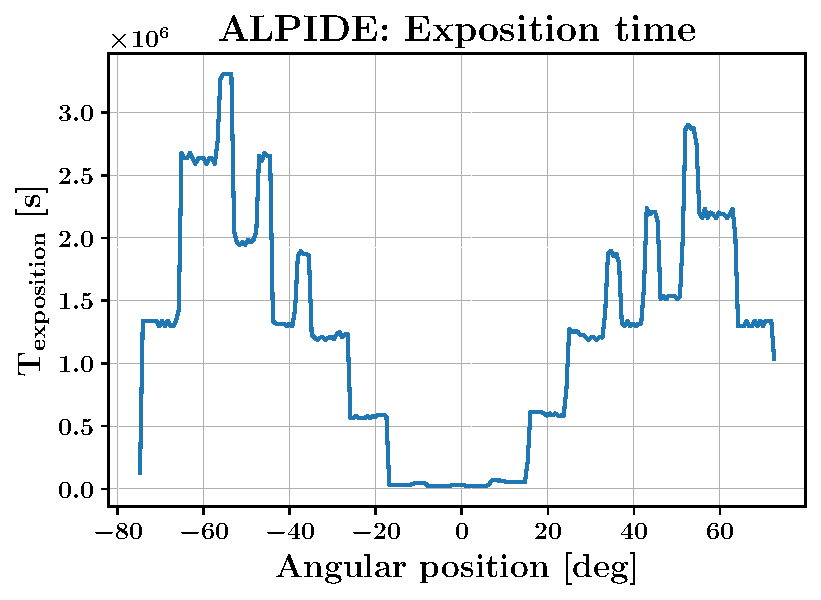
\includegraphics[width=\textwidth]{../sections/05/images/ALPIDE/ALPIDE_gold_scattering_time.pdf}
            \label{fig:time_histo}
        }
    \end{minipage}
    \hfill
    \begin{minipage}[c]{0.49\linewidth}
        \vspace{0pt}
        \centering
        \subfloat[ALPIDE total counts]{
            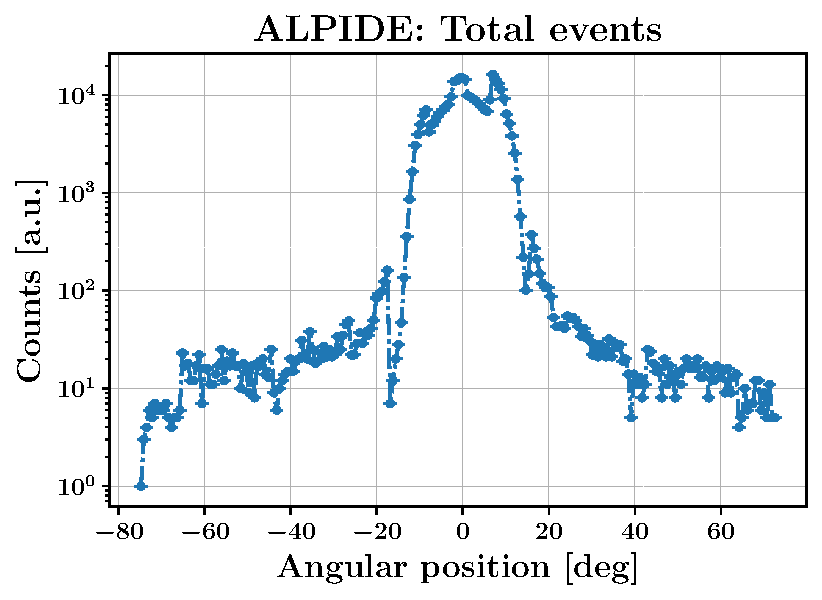
\includegraphics[width=\textwidth]{../sections/05/images/ALPIDE/ALPIDE_gold_scattering_counts.pdf}
            \label{fig:ALPIDE_counts}
        }
    \end{minipage}
    \label{fig:profile}
    \caption{ALPIDE rate normalisation on effective exposition time. In \textbf{\ref{fig:time_histo}}, the histogram of the total exposition time for the gold foil data, used as normalisation of the total angular distribution in \textbf{\ref{fig:ALPIDE_counts}}.}
\end{figure*}


The same procedure is not applied in the SSB system analysis, because of the small solid angle covered by the collimated silicon detector. In fact, the rate is evaluated for a discrete set of angles.
For this reasons, we can not directly compare the rates obtained with the two detectors, but we will treat them independently.
Hence, we present in \figref{fig:analysis_picoscope_scattering_gold} and \figref{fig:analysis_ALPIDE_scattering_gold} the final scattering distribution acquired by SSB and ALPIDE detectors, respectively, and for the gold foil. On the other hand, we present in \figref{fig:analysis_picoscope_scattering_tin} and \figref{fig:analysis_ALPIDE_scattering_tin} the final scattering distribution for both the detectors and for the tin foil.
We remark how the results with ALPIDE have a finer angular resolution even with lower acquisition times. This behaviour is due to the intrinsic properties of ALPIDE and to its higher acceptance with respect to the SSB detector. On the other hand, the SSB system offers an easier treatment of signal and background events, since it allows to sample the waveforms for each event registered.



\subsection{Statistical analysis}


\paragraph{Gold foil analysis}
Let us focus on the results for the gold foil. We immediately observe that the tails of the distributions showed in \figref{fig:analysis_picoscope_scattering_gold} and \figref{fig:analysis_ALPIDE_scattering_gold} are populated with respect to the case of the beam profile. This is a clear evidence of the fact that the \( \alpha \) particles undergo to Rutherford scattering when traversing the scattering foil. Here, we try to give statistical significance to this evidence.

In order to compare the theoretical distribution, provided by the simulation, with our experimental results, we employ two statistical tests. The first one is a standard $\chi^2$ estimator, computed as the square sum of the normalised residuals, while the second one is the Two-Sample Kolmogorov–Smirnov (KS) test. Due to the significant variation in the order of magnitude of the rate along the scattering profile, it is convenient and more reliable to conduct the tests only for the tails of the distributions, namely the angular regions with \( \theta \leq-30^{\circ} \) (left tail) and \( \theta \geq 30^{\circ} \) (right tail). The results of the tests are reported in \tabref{tab:stats}.


\begin{figure*}[!h]
    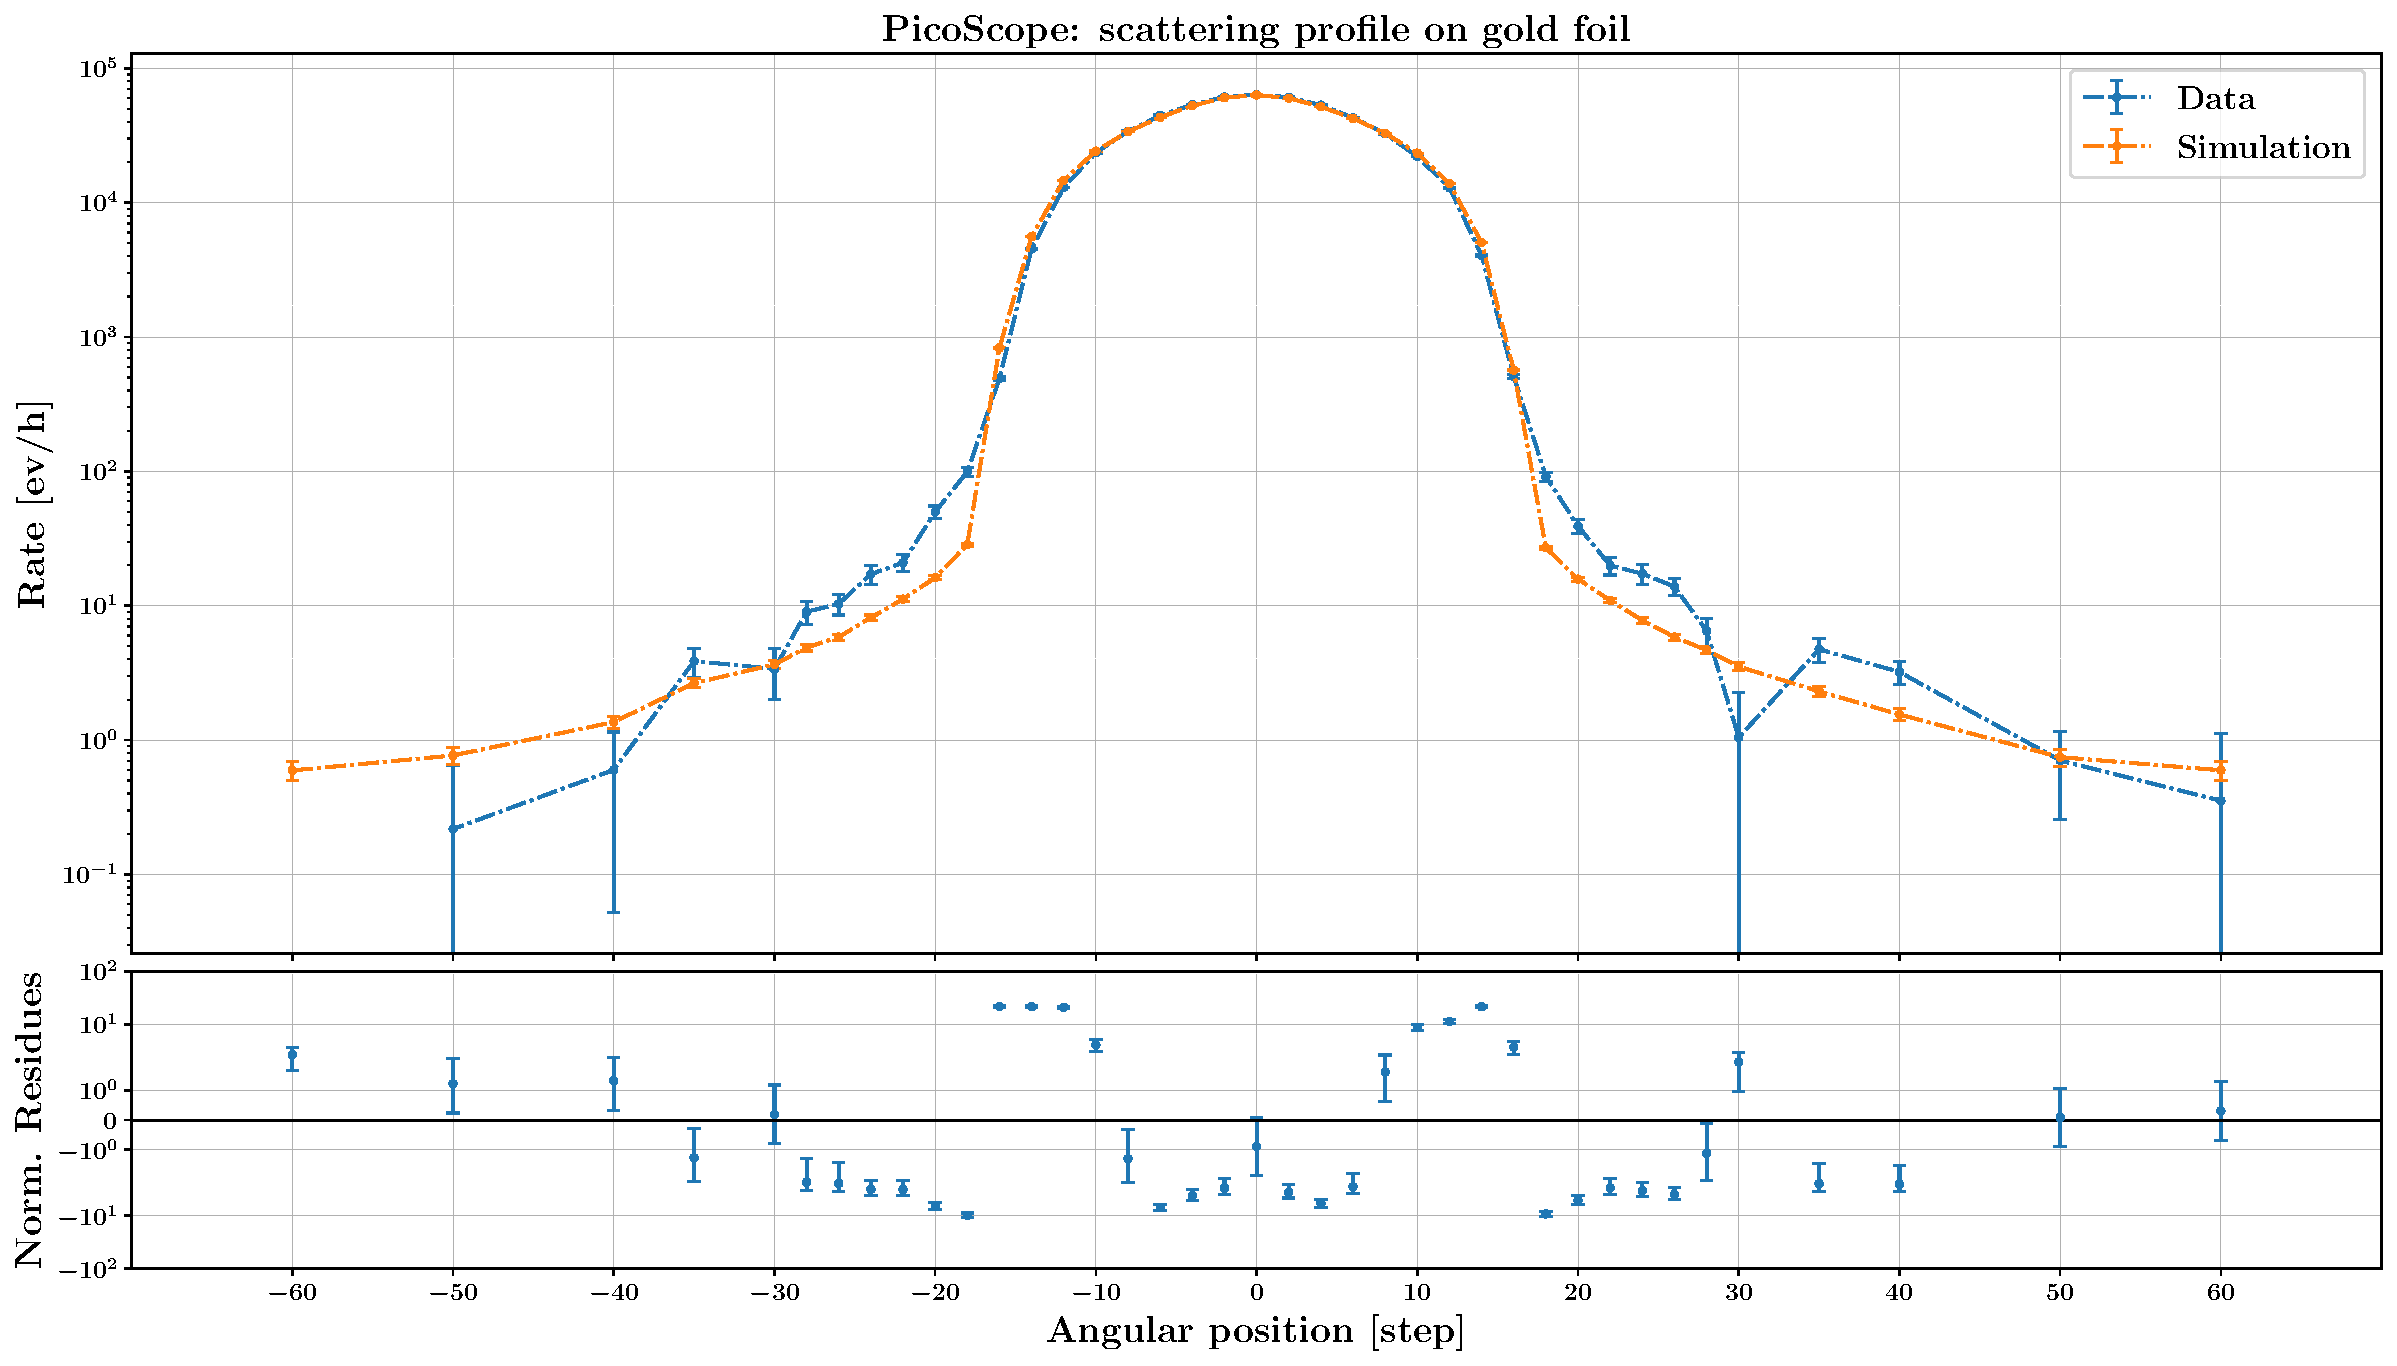
\includegraphics[width=1.0\textwidth]{\main/../sections/05/images/picoscope/gold_scattering_profile.pdf}
    \caption{Scattering angular distribution extracted from SSB system data and for a gold foil as target.}
    \label{fig:analysis_picoscope_scattering_gold}
\end{figure*}

\begin{figure*}[!h]
    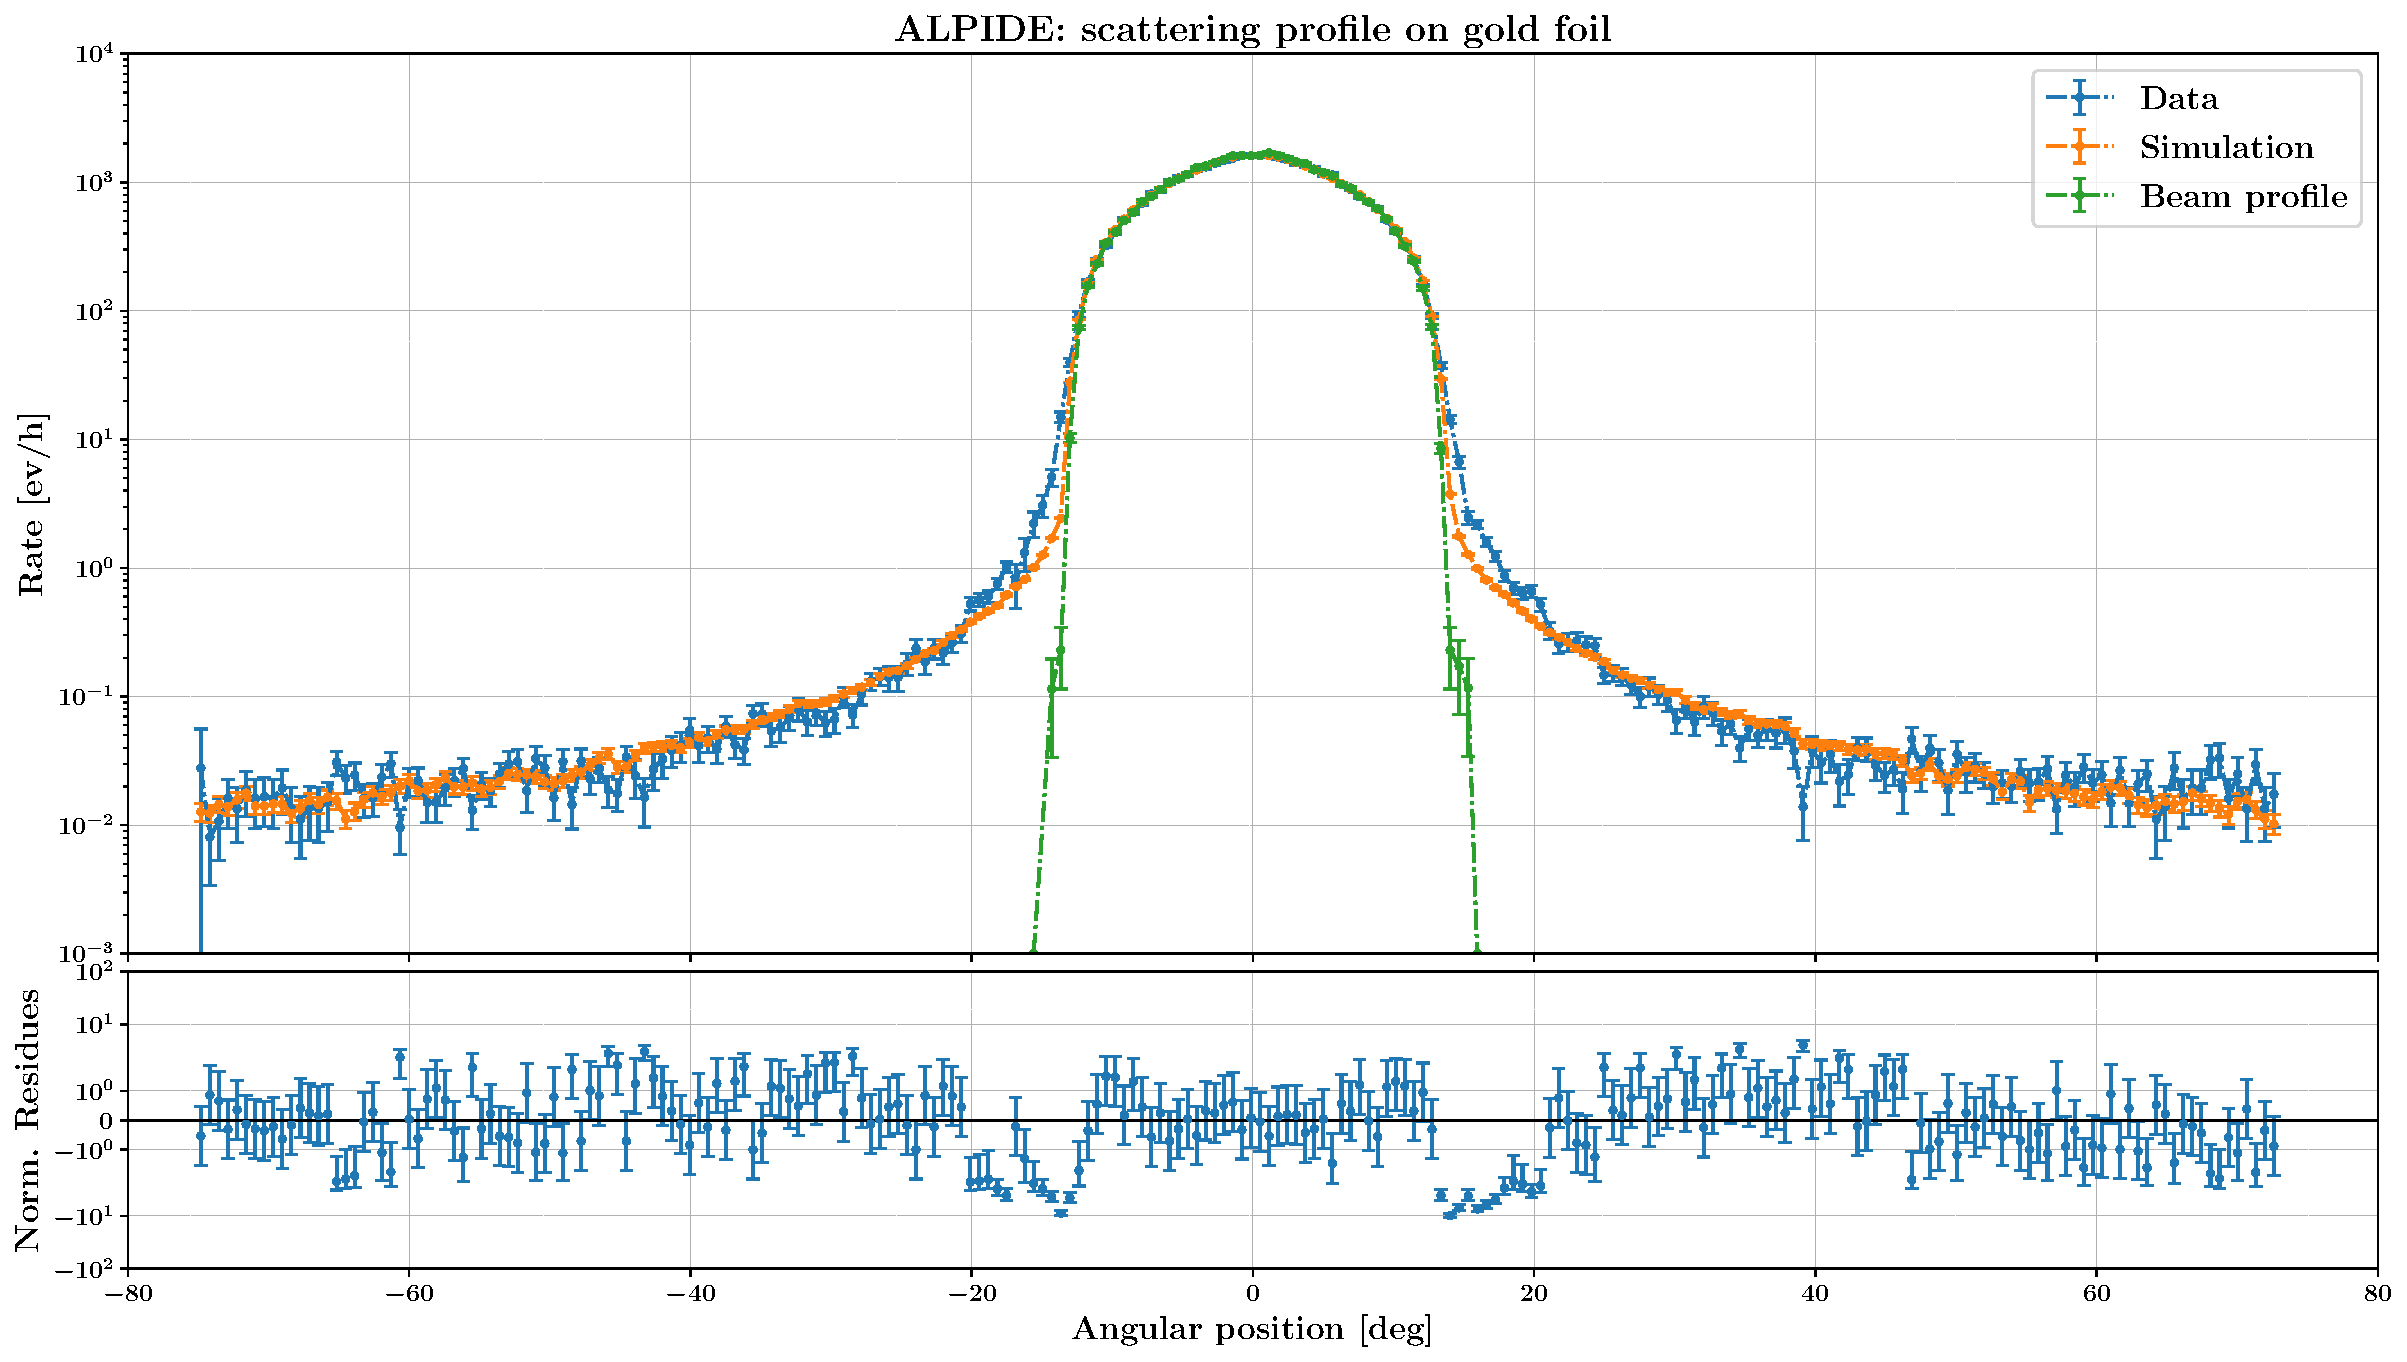
\includegraphics[width=1.0\textwidth]{\main/../sections/05/images/ALPIDE/ALPIDE_gold_scattering_profile.pdf}
    \caption{Scattering angular distribution extracted from ALPIDE system data and for a gold foil as target.}
    \label{fig:analysis_ALPIDE_scattering_gold}
\end{figure*}

\clearpage

\begin{figure*}[!h]
    \includegraphics[width=1.0\textwidth]{\main/../sections/05/images/picoscope/tin_scattering_profile.pdf}
    \caption{Scattering angular distribution extracted from SSB system data and for a tin foil as target.}
    \label{fig:analysis_picoscope_scattering_tin}
\end{figure*}

\begin{figure*}[!h]
    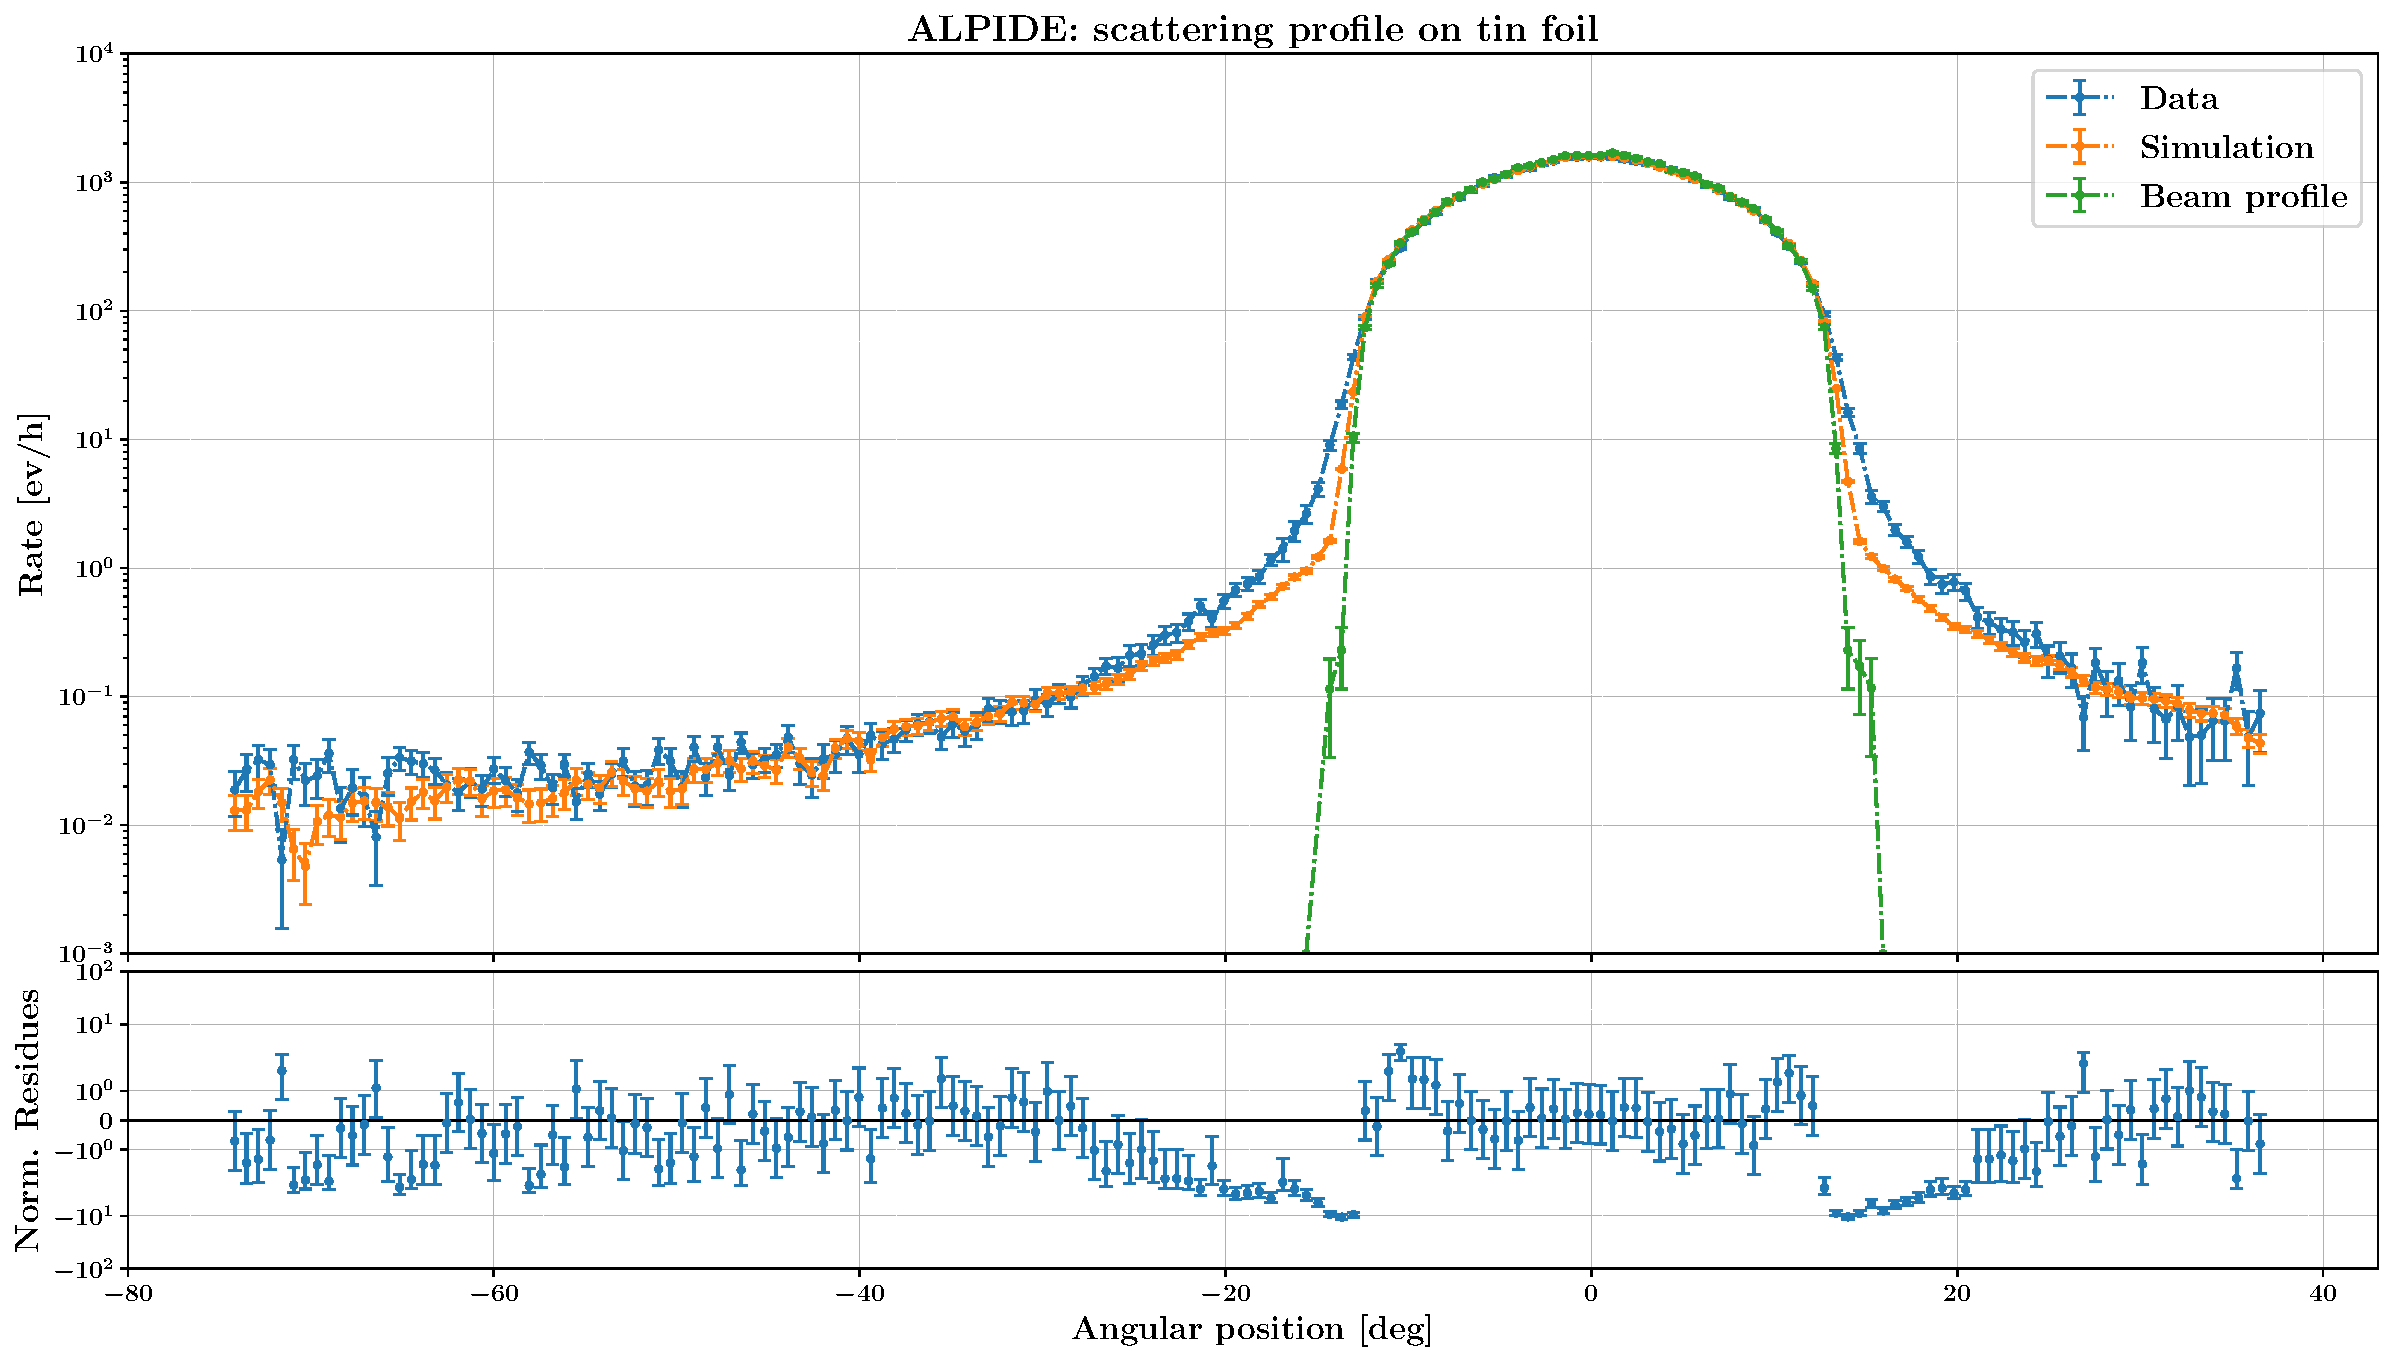
\includegraphics[width=1.0\textwidth]{\main/../sections/05/images/ALPIDE/ALPIDE_tin_scattering_profile.pdf}
    \caption{Scattering angular distribution extracted from ALPIDE system data and for a tin foil as target.}
    \label{fig:analysis_ALPIDE_scattering_tin}
\end{figure*}

\clearpage


\begin{table}[h]
    \begin{tabular}{cl|cc|ccc}
        \toprule
        \multicolumn{2}{c|}{\textbf{Distribution}} &
        \multicolumn{2}{c|}{\textbf{$\boldsymbol{\chi}^2$ test}} &
        \multicolumn{3}{c}{\textbf{KS test}}\\
        \colrule
        \textbf{Detector} & \textbf{Interval} & $\boldsymbol{\chi}^2$ &
        \textbf{n.d.f.} & $\boldsymbol{\alpha}$ & $D^{\mathrm{crit}}$
        & $D_{n,m}$\\
        \colrule
        \multirow{2}{*}{ALPIDE} & $\theta < -30^{\circ}$ & 72 & 75 & 0.05 & 0.059  & 0.055 \\
                                & $\theta > +30^{\circ}$ & 83 & 71 & 0.05 & 0.062  & 0.067 \\
        \colrule
        \multirow{2}{*}{SSB} & $\theta < -30^{\circ} $   & 5.2 & 4 & 0.05 &  0.14  & 0.09 \\
                             & $\theta > +30^{\circ} $   & 11 & 4 & 0.05 & 0.14 & 0.21 \\
        \botrule
    \end{tabular}
    \caption{Results for \( \chi^{2} \) and KS tests applied to the data in the tails of the scattering distributions, acquired with SSB and ALPIDE detectors with gold foil.}
    \label{tab:stats}
\end{table}

\paragraph{Tin foil analysis}
We repeat the same analysis and we apply the same tests to the data acquired with the tin foil. Also in this case we can observe that the tails of the distributions in \figref{fig:analysis_picoscope_scattering_tin} and \figref{fig:analysis_ALPIDE_scattering_tin} are populated with respect to the case of the beam profile. However, due to time limitations, we could acquire only the left tail with ALPIDE detector.
As for the previous case, we run a Monte Carlo simulation of the experiment as a theoretical reference for our experimental results. The results for the \( \chi^{2} \) and the KS tests are reported in \tabref{tab:statsTIN}.

%\begin{figure*}[h]
%    \includegraphics[width=1.0\textwidth]{\main/../sections/05/im%ages/ALPIDE/tin_scattering_profile.pdf}
%    \caption{ALPIDE scattered beam profile on tin foil}
%
%    \label{fig:analysis_ALPIDE_scattering_tin}
%\end{figure*}




% \begin{figure*}[h]
%     \begin{minipage}[c]{0.49\linewidth}
%         \vspace{0pt}
%         \centering
%         \subfloat[SSB scattered beam profile on tin foil]{
%               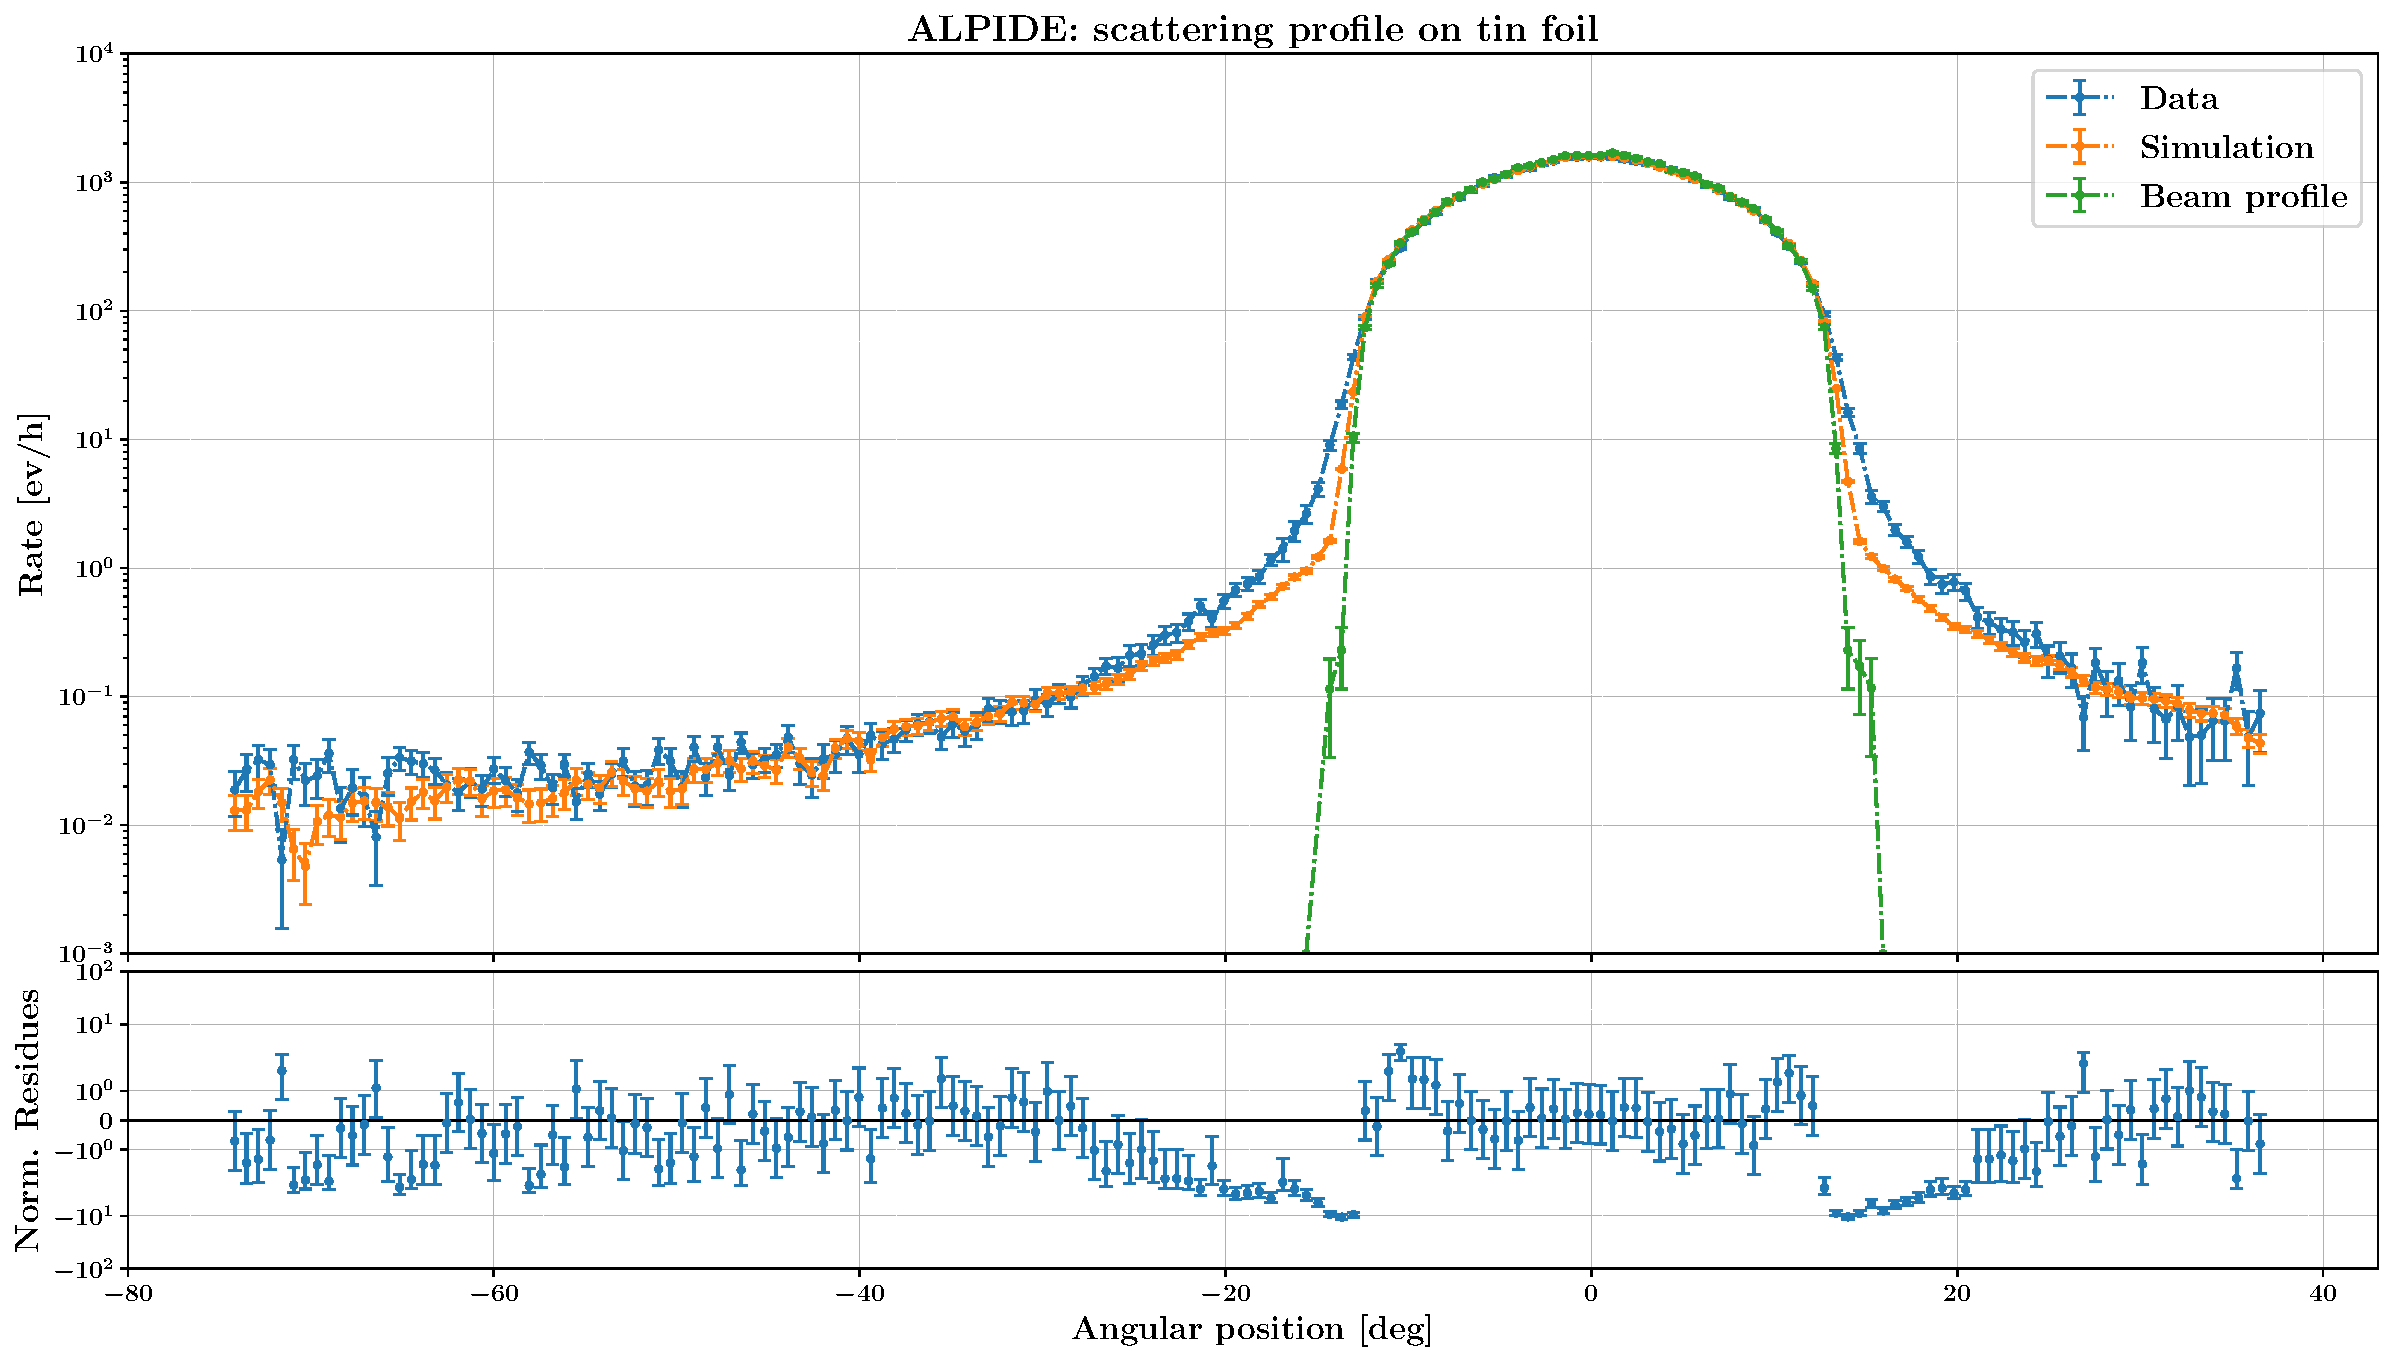
\includegraphics[width=1.0\textwidth]{\main/../sections/05/images/ALPIDE/ALPIDE_tin_scattering_profile.pdf}
%     \label{fig:analysis_PICO_scattering_tin}
%         }
%     \end{minipage}
%     \hfill
%     \begin{minipage}[c]{0.49\linewidth}
%         \vspace{0pt}
%         \centering
%         \subfloat[ALPIDE scattered beam profile on tin foil]{
%           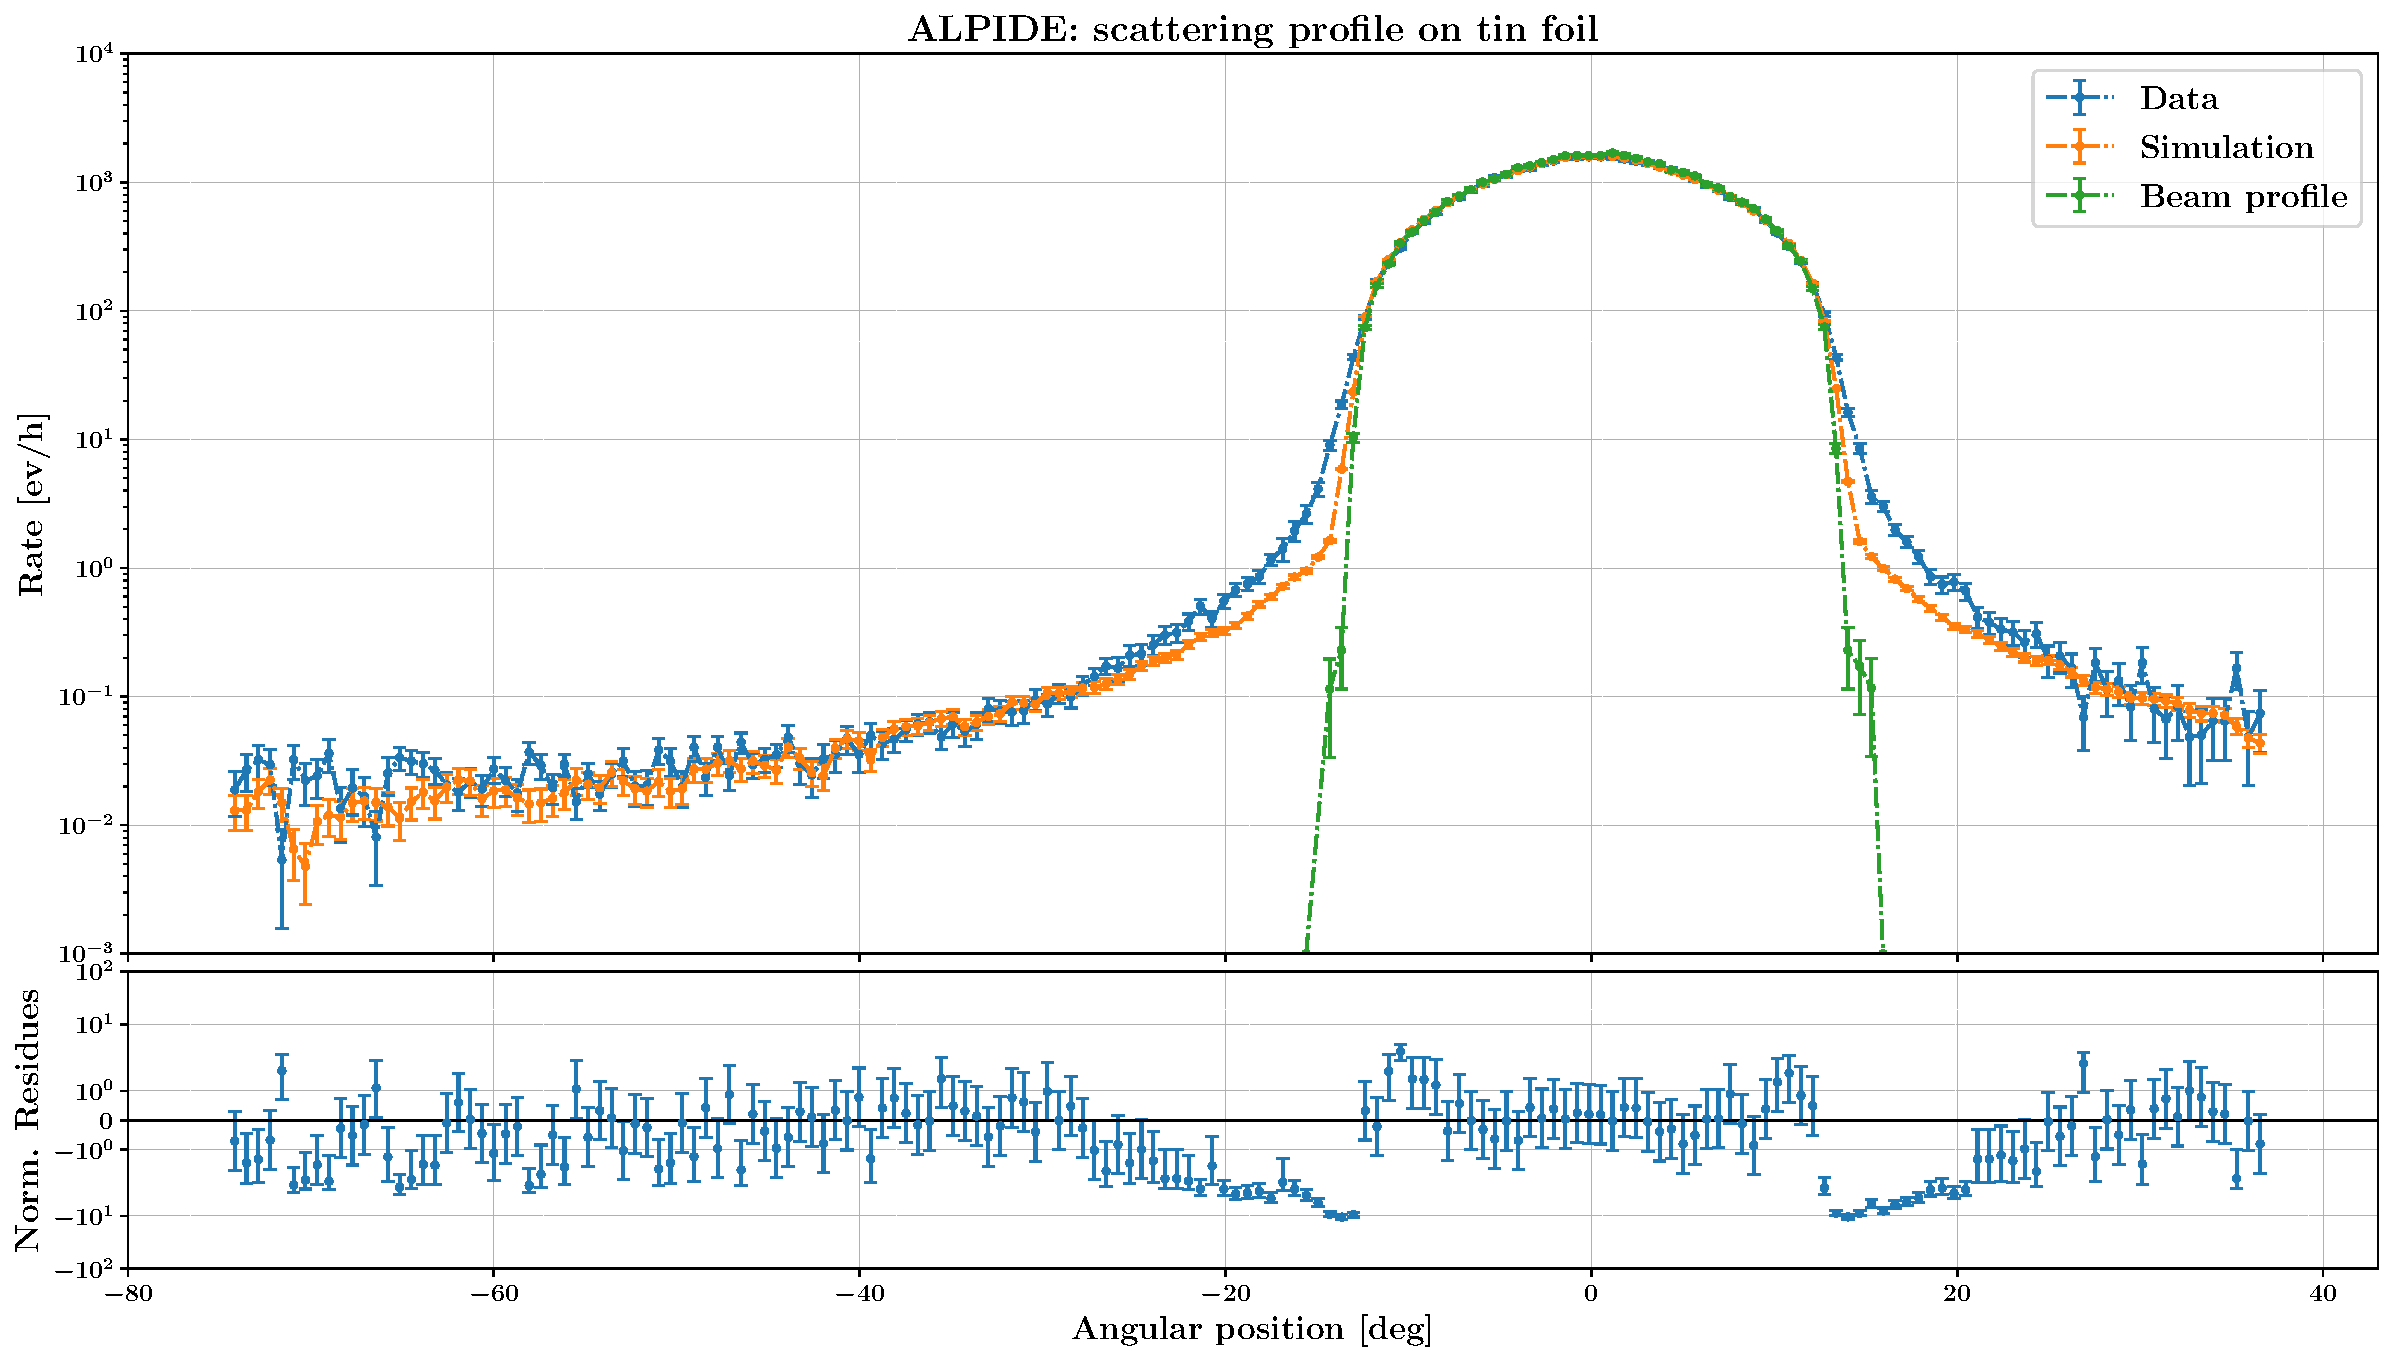
\includegraphics[width=1.0\textwidth]{\main/../sections/05/images/ALPIDE/ALPIDE_tin_scattering_profile.pdf}
%     \label{fig:analysis_ALPIDE_scattering_tin}
%         }
%         % \caption{Beam profile acquired with the silicon detector. Comparison between simulation and experimental curve}   
%     \end{minipage}
%     \label{fig:profileTIN}
%     \caption{Scattering profile of the $\alpha$ particles of the tin foil. Profile acquired using the SSB detector, in \figref{fig:analysis_PICO_scattering_tin}, and the ALPIDE detector, in \figref{fig:analysis_ALPIDE_scattering_tin}.}
% \end{figure*}


\begin{table}[h]
    \begin{tabular}{cl|cc|ccc}
        \toprule
        \multicolumn{2}{c|}{\textbf{Distribution}} &
        \multicolumn{2}{c|}{\textbf{$\boldsymbol{\chi}^2$ test}} &
        \multicolumn{3}{c}{\textbf{KS test}}\\
        \colrule
        \textbf{Detector} & \textbf{Interval} & $\boldsymbol{\chi}^2$ &
        \textbf{n.d.f.} & $\boldsymbol{\alpha}$ & $D^{\mathrm{crit}}$
        & $D_{n,m}$\\
        \colrule
        \multirow{2}{*}{ALPIDE} & $\theta < -30^{\circ} $ & 87 & 75 & 0.05 & 0.061  & 0.058 \\
                                & $\theta > +30^{\circ} $ & \( *** \) & \( *** \) & \( *** \)  & \( *** \)   & \( *** \)  \\
        \colrule
        \multirow{2}{*}{SSB }   & $\theta < -30^{\circ} $ & 7.9 & 3 &0.05 & 0.17 & 0.21 \\
                                & $\theta > +30^{\circ} $ & 4.2 & 3 &0.05 & 0.17 & 0.16 \\
        \botrule
    \end{tabular}
    \caption{Results for \( \chi^{2} \) and KS tests applied to the data in the tails of the scattering distributions, acquired with SSB and ALPIDE detectors with tin foil.}
    \label{tab:statsTIN}
\end{table}



\subsection{Discussion of results}
As it is possible to observe from all the scattering distributions, there is a always a small deviation of experimental data from the simulated distribution around the region of \( \sim \abs{\theta} = 20^{\circ} \). Let us focus on the physical motivation of this phenomenon. What happens in a real experiment is that some \( \alpha \) particles arriving at the border of the final second collimator of the beam are not stopped, but only braked, and so they continue to travel to the detector. In the simulation we do not consider this behaviour since for the final analysis we are interested only in the tail regions, namely to \( \abs{\theta} \geq 30^{\circ} \). Another factor not considered in the simulation is the multiple scattering, but this is a second order effect for this type of analysis, so we ignore it.

We return now to the final analysis and to the results of the statistical tests. Focusing on the gold foil dataset, we observe from \tabref{tab:stats} that there is a good agreement between the expected results and the acquired ones for both the tails for ALPIDE detector and only for the left tail for SSB detector. On the other hand, for the tin foil dataset, we find a good agreement only for ALPIDE on the left tail, while for the other cases we find some discrepancies.

For both the foils, the deviations from the expected distribution may be caused by the low statistics acquired by the SSB detector, affected by a very low acceptance value. On the other hand, the simulation should be improved in order to take into account more realistically the microscopic structure of the foil, for example by including the metal structure. Another factor that may influence the statistical results is the eventuality of an imperfect alignment of the detectors in the transverse direction with respect to the beam. Further analysis in this sense should be done in the future iterations of the experiment. Last but not least, higher statistics of acquisition should be chosen in order to smooth the angular distributions and reduce the statistical fluctuations. This was not possible during this year iteration due to the limited amount of time at our disposal.


% As we can see the angular scattering plot, shown in \textbf{ref figure alpide} \figref{fig:analysis_PICO_scattering_tin}, presents a small deviation from the simulated profile in the regions around $|\theta |=20$. This deviation can be explained as the result of some second order effects which we did not considered in the simulation, such as the possible scattering of the particles on the collimator border and the multiple scattering in the interaction with the target. We are however more interested in the comparison in the tail regions,  which are the direct manifestation of the Rutherford scattering. As we can see from the statistical analysis reported in \tabref{tab:stats} and \tabref{tab:statsTIN} there is a very good agreement between simulation and experiment in the left tail ($|\theta| \leq -30$) while the right tail ($|\theta| \geq 30$) present a less ideal agreement, especially for the data acquired using the SSB detector. This behaviour is however expected since at high angles we are highly influenced by statistical fluctuations and background events which become really relevant due to the small statistic. 
% Another factor that may have influenced the statistical results is the possibility of a non perfect alignment of the ALPIDE detector in the transverse direction respect to the beam.

% A deeper analysis of this comparison may be conducted but would require longer acquisition times at higher angles, which was not possible is our temporal window. 

% The results are however still very good since we are able to see the effects of the Rutherford scattering and also able to efficiently simulate them with good precision as we saw before.


\end{document}
